\chapter{Introduction}

Global Navigation Satellite Systems, GNSS for short, are uesd in a wide variety of applications nowadays.
The most prominent and oldest system is GPS.
It started as a military and maritime navigation aid, but is now used extensively in civil applications.
This thesis evaluates the use of GPS for the localization of a sounding rocket.

\section{Framework}

The need for such a project originated form ARIS, the Swiss Space Initiative or Akademische Raumfahrt Initiative Schweiz in german.
ARIS was founded in 2017 by students from the ETH Z\"urich and HSLU.
Now, over 50 students from the ETH Z\"urich and the universities of applied sciences in Luzern (HSLU) and Z\"urich (ZHAW) work on its inaugural project which is called TELL.
The goal of project TELL is to build a sounding rocket to compete in the 2018 Spaceport America Cup in New Mexico.
More than 100 student teams compete there to launch a 4kg payload with a sounding rocket to a target altitude of 10000 feet or about 3km. \cite{aris}

\noindent
\begin{minipage}{0.5\textwidth}
 \centering
 
\includegraphics[height=5.5cm]{images/Tell_Logo.png}
 \captionof{figure}{Project Tell}
\end{minipage}
\begin{minipage}{0.5\textwidth}
 \centering
 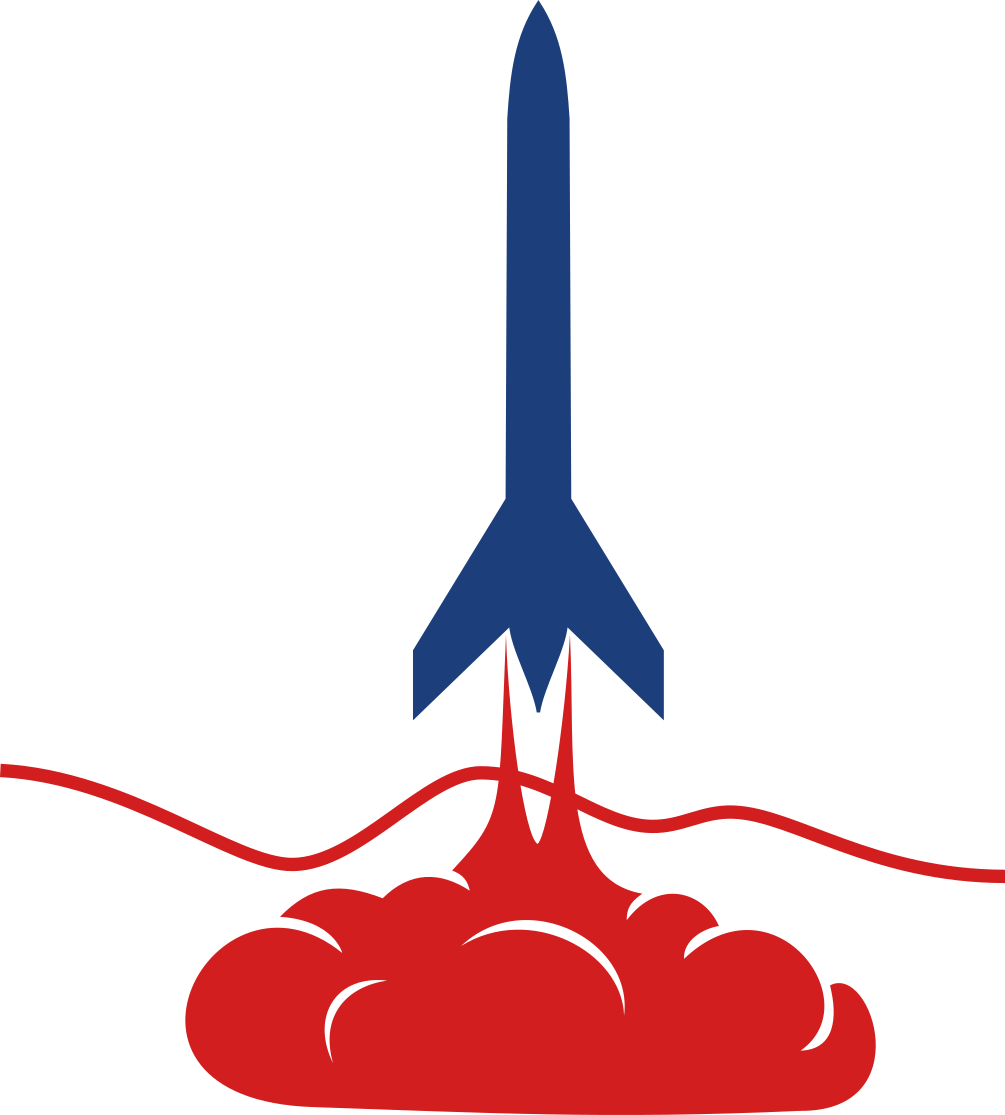
\includegraphics[height=5.5cm]{images/SAC_Logo.png}
 \captionof{figure}{Spaceport America Cup}
\end{minipage}

\vspace{0.5cm}

A jury distributes points for achievements in the competition itself and the planning, engineering and documentation that went into the project.
A maximum score of 1000 points can be reached.
The points are distributed as follows:
\begin{itemize}
 \item Delivery of Entry Form: 60 points - 6\%
 \item Technical Report: 200 points - 20\%
 \item Design Implementation: 240 points - 24\%
 \item Flight Performance: 500 points - 50\%
\end{itemize}

Points for flight performance are split between reached apogee relative to the target apogee (350 points) and successful recovery (150 points).
The points for apogee precision are calculated with this formula:
$$ Points = 350 - \left( \frac{350}{0.3 \times Apogee_{Target}} \right) \times \abs{Apogee_{Target} - Apogee_{Actual}} $$
$$ \text{with } Apogee_{Target} = 3048m(10000feet)$$ 

With that equation, a deviation of about 9 meters from the target apogee results in a loss of 1\% (3.5 points) of possible points for a correct apogee. \cite{sac_rules2017}

For project TELL, the rocket motor is dimensioned to overshoot the target apogee and airbrakes are used to reduce the apogee to the target.
A controll loop is implemented to controll the position of the airbrakes during the accent.
The position and velocity data for the loop is fused from on-board pressure and acceleration sensors.
Although GPS is implemented in the rocket, it is only used to locate and recover the rocket after it landed.
This is because standalone GPS has a vertical error of less than 15 meters for 95\% of the time. \cite{SPS_Performance}
This is not accurate enouth to be beneficial for the sensor fusion.
A vertical error of less than 1 meter for 95\% of the time would be needed for it to be feasable.
With such an accuracy improvement, the GPS position could be fused together with the pressure and accelerometer.
The addition of GPS would especcialy help in reducing the drift introduced by the accelerometer.
This is the origin of this bachelor thesis.


\section{Task Decsription}

In short, the feasability of GPS for the localization of a sounding rocket should be evaluated.
This should be done in multiple steps.
First, it has to be determined which internal and external error sources could limit the GPS accuracy.
This means errors that degrade the GPS signal before it enters the antenna, as well as errors that come from the signal processing.
A focus should be on potential error sources that are specific to the application in a sounding rocket.

Based on that, methods to mitigate those errors should be found.
These methods should be feasable to implement in a sounding rocket and enhance the accuracy of the GPS positioning to a level where it is usable for the rocket controll.
The fasability of one of the methods should be shown with a proof of concept.
That could be a simulation or a prototype depending on the approach.


\section{Requirements}\label{Requirements}

To make it possible to integrate the approach into the rocket, a set of requirements is defined.
Also requirements for the performance of the system are given.
